\begin{figure}[H]
    \begin{subfigure}[t]{.3\textwidth}
        \caption{}
        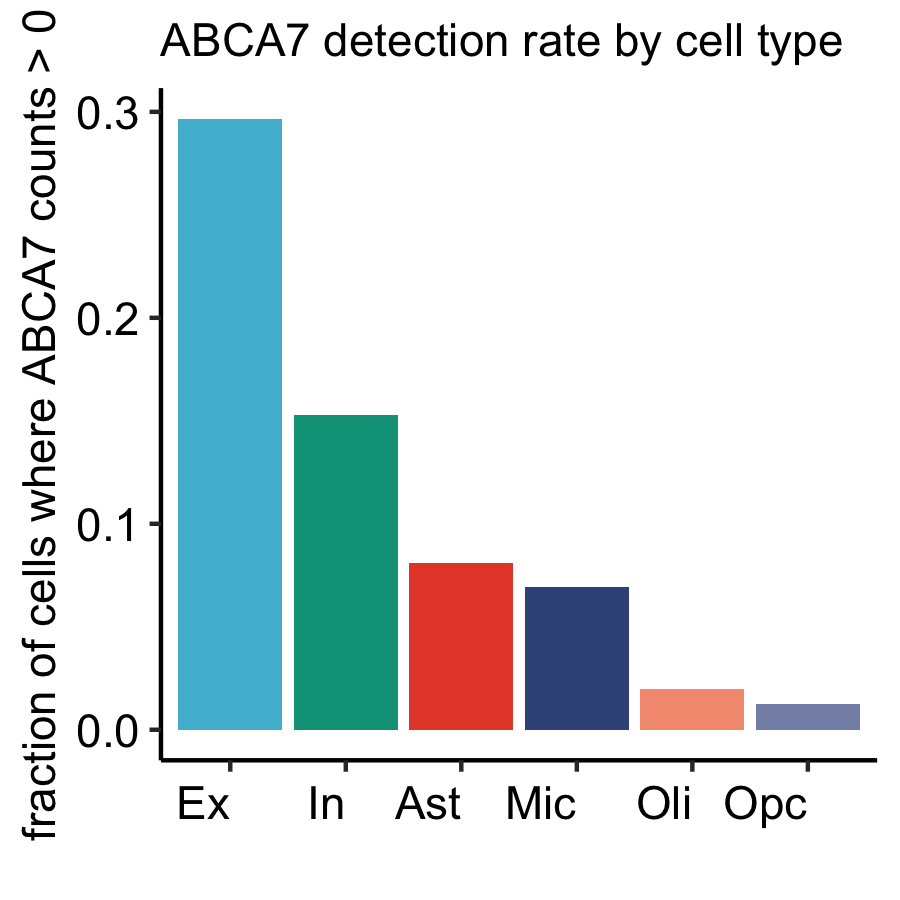
\includegraphics[width=\textwidth]{./extended_plots/abca7_detection_rate.png}        
    \end{subfigure}
    \par
    \begin{subfigure}[t]{1\textwidth}
        \caption{}
        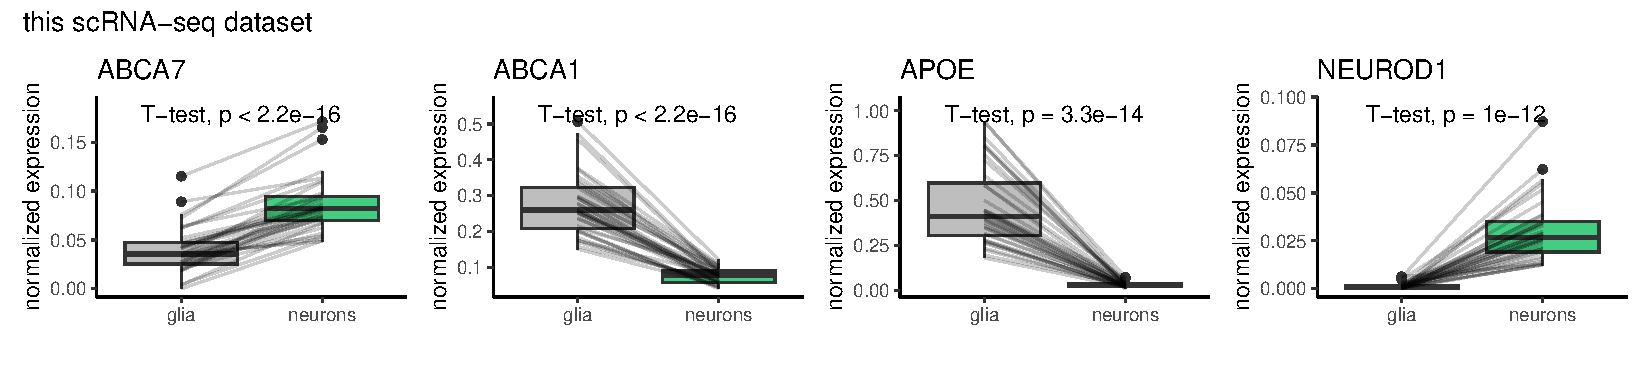
\includegraphics[width=\textwidth]{./extended_plots/scRNAseq_bulk_rna.pdf}        
    \end{subfigure}
    \begin{subfigure}[t]{1\textwidth}
        \caption{}
        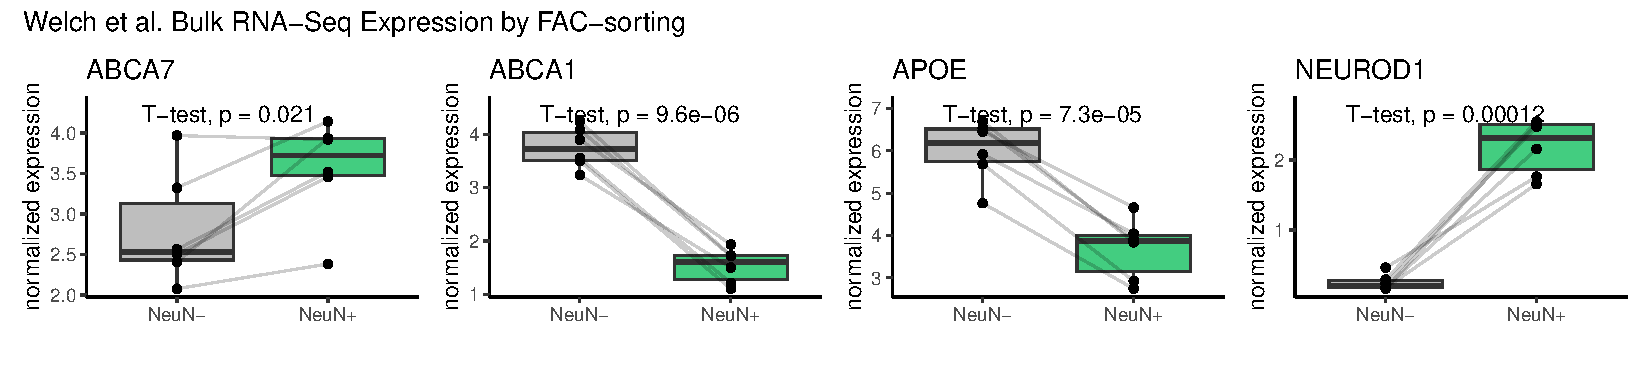
\includegraphics[width=\textwidth]{./extended_plots/welch_et_al_bulk_rna.pdf}        
    \end{subfigure}
    \caption{
        \textbf{Neuronal Expression of ABCA7 in the Post-mortem Human Brain.}\\
    }
    \label{fig:abca7_expression}
\end{figure}
\begin{itemize}
    \item[\textbf{(A)}] Per cell type ABCA7 detection rate of major cell types in the post-mortem PFC as quantified by snRNA-seq. 
    \item[\textbf{(B)}] Normalized expression of indicated gene in glial cells (per-individual mean expression profiles across Oli, Opc, Ast, Mic) vs. neuronal cells (per-individual mean expression profiles across Ex and In) from post-mortem snRNA-seq data. 
    \item[\textbf{(C)}] Normalized expression of indicated genes in NeuN- vs. NeuN+ cells (N=6 individuals, from \cite{Welch2022-aa}; see Table 2). All p-values are computed by paired two-sided t-test. Boxes indicate per-condition dataset quartiles, and whiskers extend to the most extreme data points not considered outliers (i.e., within 1.5 times the interquartile range from the first or third quartile).
\end{itemize}